%---------- Inleiding ---------------------------------------------------------
\chapter{Bijlage bij WikiSQL}
\label{ch:bijlage1}
\section{Vraag, Query en Tabel} % The \section*{} command stops section numbering
\begin{figure}[htb]
	\centering
	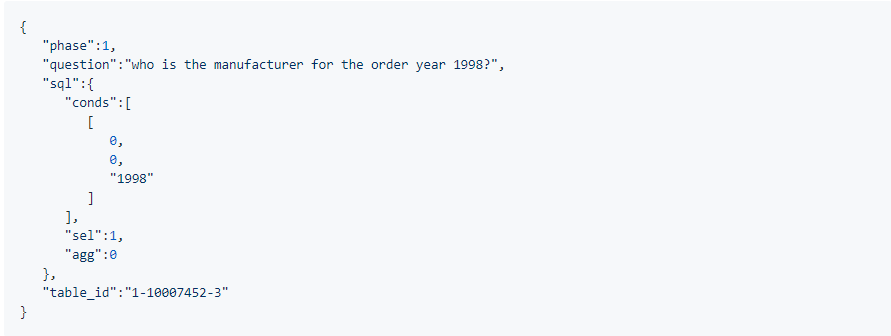
\includegraphics[width=1\textwidth]{img/vraag}
	\caption[WikiSQL Vraag, Query en Tabel]{WikiSQL Vraag, Query en Tabel}
\end{figure}
\break
\section{Tabellen} % The \section*{} command stops section numbering
\begin{figure}[htb]
	\centering
	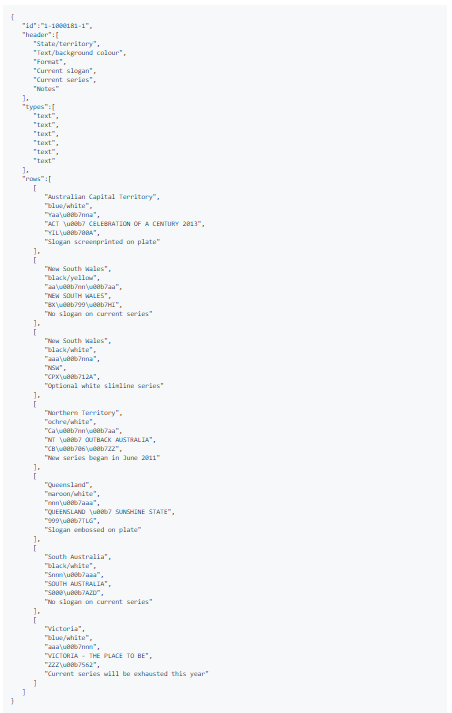
\includegraphics[width=0.7\textwidth]{img/tabel}
	\caption[WikiSQL Tabellen]{WikiSQL Tabellen}
\end{figure}